\documentclass[../main.tex]{subfiles}
\hbadness=1000000
\vbadness=1000000

\begin{document}
\section{Introduction}
In this chapter, we cover the study we conducted on information transmission in cortical circuits.
This work was materialized in the scientific publication bearing the same title as this chapter: \textit{Information transmission in delayed neuronal circuits in the presence of a relay population} \citep{sanchez-claros_information_2021}.
The main characteristic that displays these types of circuits is that they can exhibit zero-lag synchronization despite involving spatially distant areas; in other words, there are non-negligible delays.
Therefore, a fundamental piece of the work in this chapter is synchronization, and the fundamental question that motivated us is under what conditions a network exhibiting zero-time synchronization can efficiently transmit information.

\subsection{Synchronization in cortical networks}
Synchronization is a fascinating phenomenon that lies at the heart of the complex dynamics and information processing of the brain. 
It refers to the coordinated firing of neurons and oscillatory activity in brain networks \citep{buzsaki_large-scale_2004}, which is believed to play a crucial role in various cognitive processes, including perception, attention, working memory, and motor function \citep{singer_binding_2007, coll_behavioral_2018,opitz_neural_2010,niebur_electrophysiological_2002,borisyuk_oscillatory_1999, doesburg_large-scale_2008,baddeley_working_1992,baddeley_working_2010,denker_phase_2007,baker_synchronization_2003, feige_dynamic_2000}.
The phenomenon of synchronization between neural populations is a prevalent feature in brain circuits, leading to brain oscillations across different frequency ranges \citep{pfurtscheller_brain_2000, basar_brain_2000, varela2001brainweb, basar_brain_2012, jensen_human_2019}.
Coherence and phase relations between oscillations in distinct brain regions have been proposed to modulate information transmission and directionality \citep{eckhorn_coherent_1988, pfurtscheller_brain_2000,gross_dynamic_2001,fries_mechanism_2005,maris_diverse_2016}.

\subsubsection{Zero-lag synchronization}
One intriguing case of synchronization involves zero-lag synchronization between distant cortical areas 
\citep{esfahani_zero-lag_2014,gollo_mechanisms_2014,vicente_dynamical_2008,chawla_zero-lag_2001,viriyopase_when_2012}.
The first studies on this topic showed experimental evidence that the relative phase of gamma oscillations in widely separated brain areas is approximately zero \citep{frien1994stimulus, roelfsema_visuomotor_1997,castelo1998synchronization, rodriguez1999perception,gross2004modulation}.
This result was remarkable in the presence of considerable delays due to axonal conduction and synaptic transmission.
This phenomenon was the subject of controversy due to the challenge of achieving zero-lag synchronization despite non-negligible connection delays \citep{vicente_dynamical_2008,viriyopase_when_2012}.
It has been shown in several publications that two mutually coupled systems with delay rarely synchronize at zero lag. \citep{ernst1995synchronization,ernst1998delay,goel2002synchrony,zeitler2009asymmetry}.
Fischer \textit{et al.} \citep{fischer_zero-lag_2006} and Vicente \textit{et al.} \citep{vicente_dynamical_2008} proposed a mechanism called dynamical relaying, which allows two distant neural populations to synchronize with zero delay if a third element acts as a relay between them.
This structure of three elements is commonly called a V-motif, and after its proposal, several computational studies have been performed to elucidate its properties \citep{fischer_zero-lag_2006,uhlhaas_neural_2009,esfahani_zero-lag_2014,mirasso_anticipated_2017}.
This mechanism has important biological relevance, especially in cortico-thalamic loops, where the thalamus acts as an intermediate (relaying) element indirectly connecting cortical regions \citep{sysoeva_thalamo-cortical_2016, save_hippocampal-parietal_2000,sherman_thalamocortical_2012,uhlhaas_neural_2006,theyel2010corticothalamocortical}.

The addition of a cortico-cortical connection, which is crucial in cortical circuits, transforms the V-motif into a circular motif (C-motif).
In biological cortico-thalamic circuits, there is a direct cortico-cortical interaction.
For example, indirect transthalamic pathways that connect to individual postsynaptic cells in layer 4 of the cortex play an important role in information transmission between areas \citep{sherman_thalamus_2016,theyel2010corticothalamocortical}.

The concept of motif was introduced by Milo in 2002 \citep{milo2002network}, whose definition was \textit{patterns of interconnections occurring in complex networks at numbers that are significantly higher than those in randomized networks}.
In neuroscience, motifs present stereotypical arrangements of connections between groups of neurons, playing a crucial role in shaping the functional properties and information-processing capabilities of neural circuits.
Structural motifs quantify anatomical building blocks, whereas functional motifs represent elementary processing modes of a neural network.
For example, within the visual cortex, one of the most prevalent motifs comprises three elements.
This configuration likely underpins computational processes within the visual system, fostering zero-lag synchrony between distant cortical regions \citep{sporns_motifs_2004}.
Then, understanding the presence and role of motifs within networks can shed light on the fundamental principles of brain function.
\clearpage
\subsubsection{The potential role of synchronization}
To understand the cognitive processes that underlie our conscious experience, two important hypotheses have emerged: \textbf{Binding by Synchrony} and \textbf{Communication through Coherence}.

The \textbf{Binding by Synchrony} (BBS) hypothesis posits that the brain employs synchronization as a mechanism to bring together disparate neural activities and bind them into coherent representations.
This notion suggests that when different brain regions engage in synchronous oscillatory activity, they effectively coordinate their firing patterns, enabling the integration of sensory, motor, and cognitive information \citep{singer_binding_2007}.
This process is believed to facilitate the perception of a unified reality, allowing us to effortlessly combine various sensory modalities and form a seamless perception of our surroundings.
The exploration of binding by synchrony not only delves into the intricacies of how our brain weaves together the fabric of conscious experience, but also holds implications for understanding disorders characterized by impaired sensory integration and perceptual binding.

On the other hand, \textbf{Communication through Coherence} (CTC) hypothesis illuminates how synchronization plays a pivotal role in the effective transmission of information across distributed brain regions.
Through the entrainment of oscillatory rhythms, neural populations can establish temporal windows of opportunity during which communication is optimized.
Coherence, manifested as synchronous oscillations, allows neural ensembles to align their firing patterns, enhancing the efficiency of information exchange and enabling the coordinated execution of cognitive functions \citep{fries_mechanism_2005,sancristobal_role_2014,fries_rhythms_2015}.
CTC hypothesis suggests that when two brain regions need to communicate and exchange information, their neural oscillations become synchronized or coherent in a precise phase, allowing for more efficient and reliable information transfer.
Therefore, this hypothesis imposes an important constraint of perfect match of the phase difference $\Delta\phi$, axonal conduction delay $\tau_\text{axo}$ and the oscillatory frequency $f$, which should fulfill the condition \citep{fries_mechanism_2005,sancristobal_role_2014}:
\begin{equation}
    \Delta\phi = 2\pi f\tau_\text{axo}.
    \label{eq:CTC-condition}
\end{equation}
When this relation between the emitting and receiving populations is satisfied, spikes fired in the emitting population at a specific phase of the signal %(\textit{i.e.}, at the troughs of the local field potential \textcolor{red}{Los valles no son los mínimos de excitabilidad? O no entiendo la frase...}, corresponding to the excitability maxima)
arrive at the receiving population at the same phase.
This synchronous arrival triggers a maximal response in the receiving area, leading to effective communication.
However, if the phase difference $\Delta\phi$ does not satisfy the specified relationship or varies randomly, effective communication will not be achieved.
In that case, the input from a sending group would repeatedly miss the excitable phase of the receiving population oscillation.
This is schematically represented in Figure \ref{fig:CTC}, where red and green populations stage a scenario of effective communication, and, in contrast, black and green populations represent the scenario of no communication.
Therefore, according to this hypothesis, it is possible to adjust the phase relationship between two regions to activate and deactivate communication channels \citep{fries_rhythms_2015, fries_mechanism_2005,womelsdorf2006neuronal,womelsdorf_modulation_2007}.
The diversity and time dependence of phase relationships observed in experiments \citep{womelsdorf2006neuronal,tiesinga2010mechanisms,van2015both,maris_diverse_2016} contribute to the various communication patterns in neural circuits, \textit{i.e.}, different windows for effective information transmission.
\begin{figure}
    \centering
    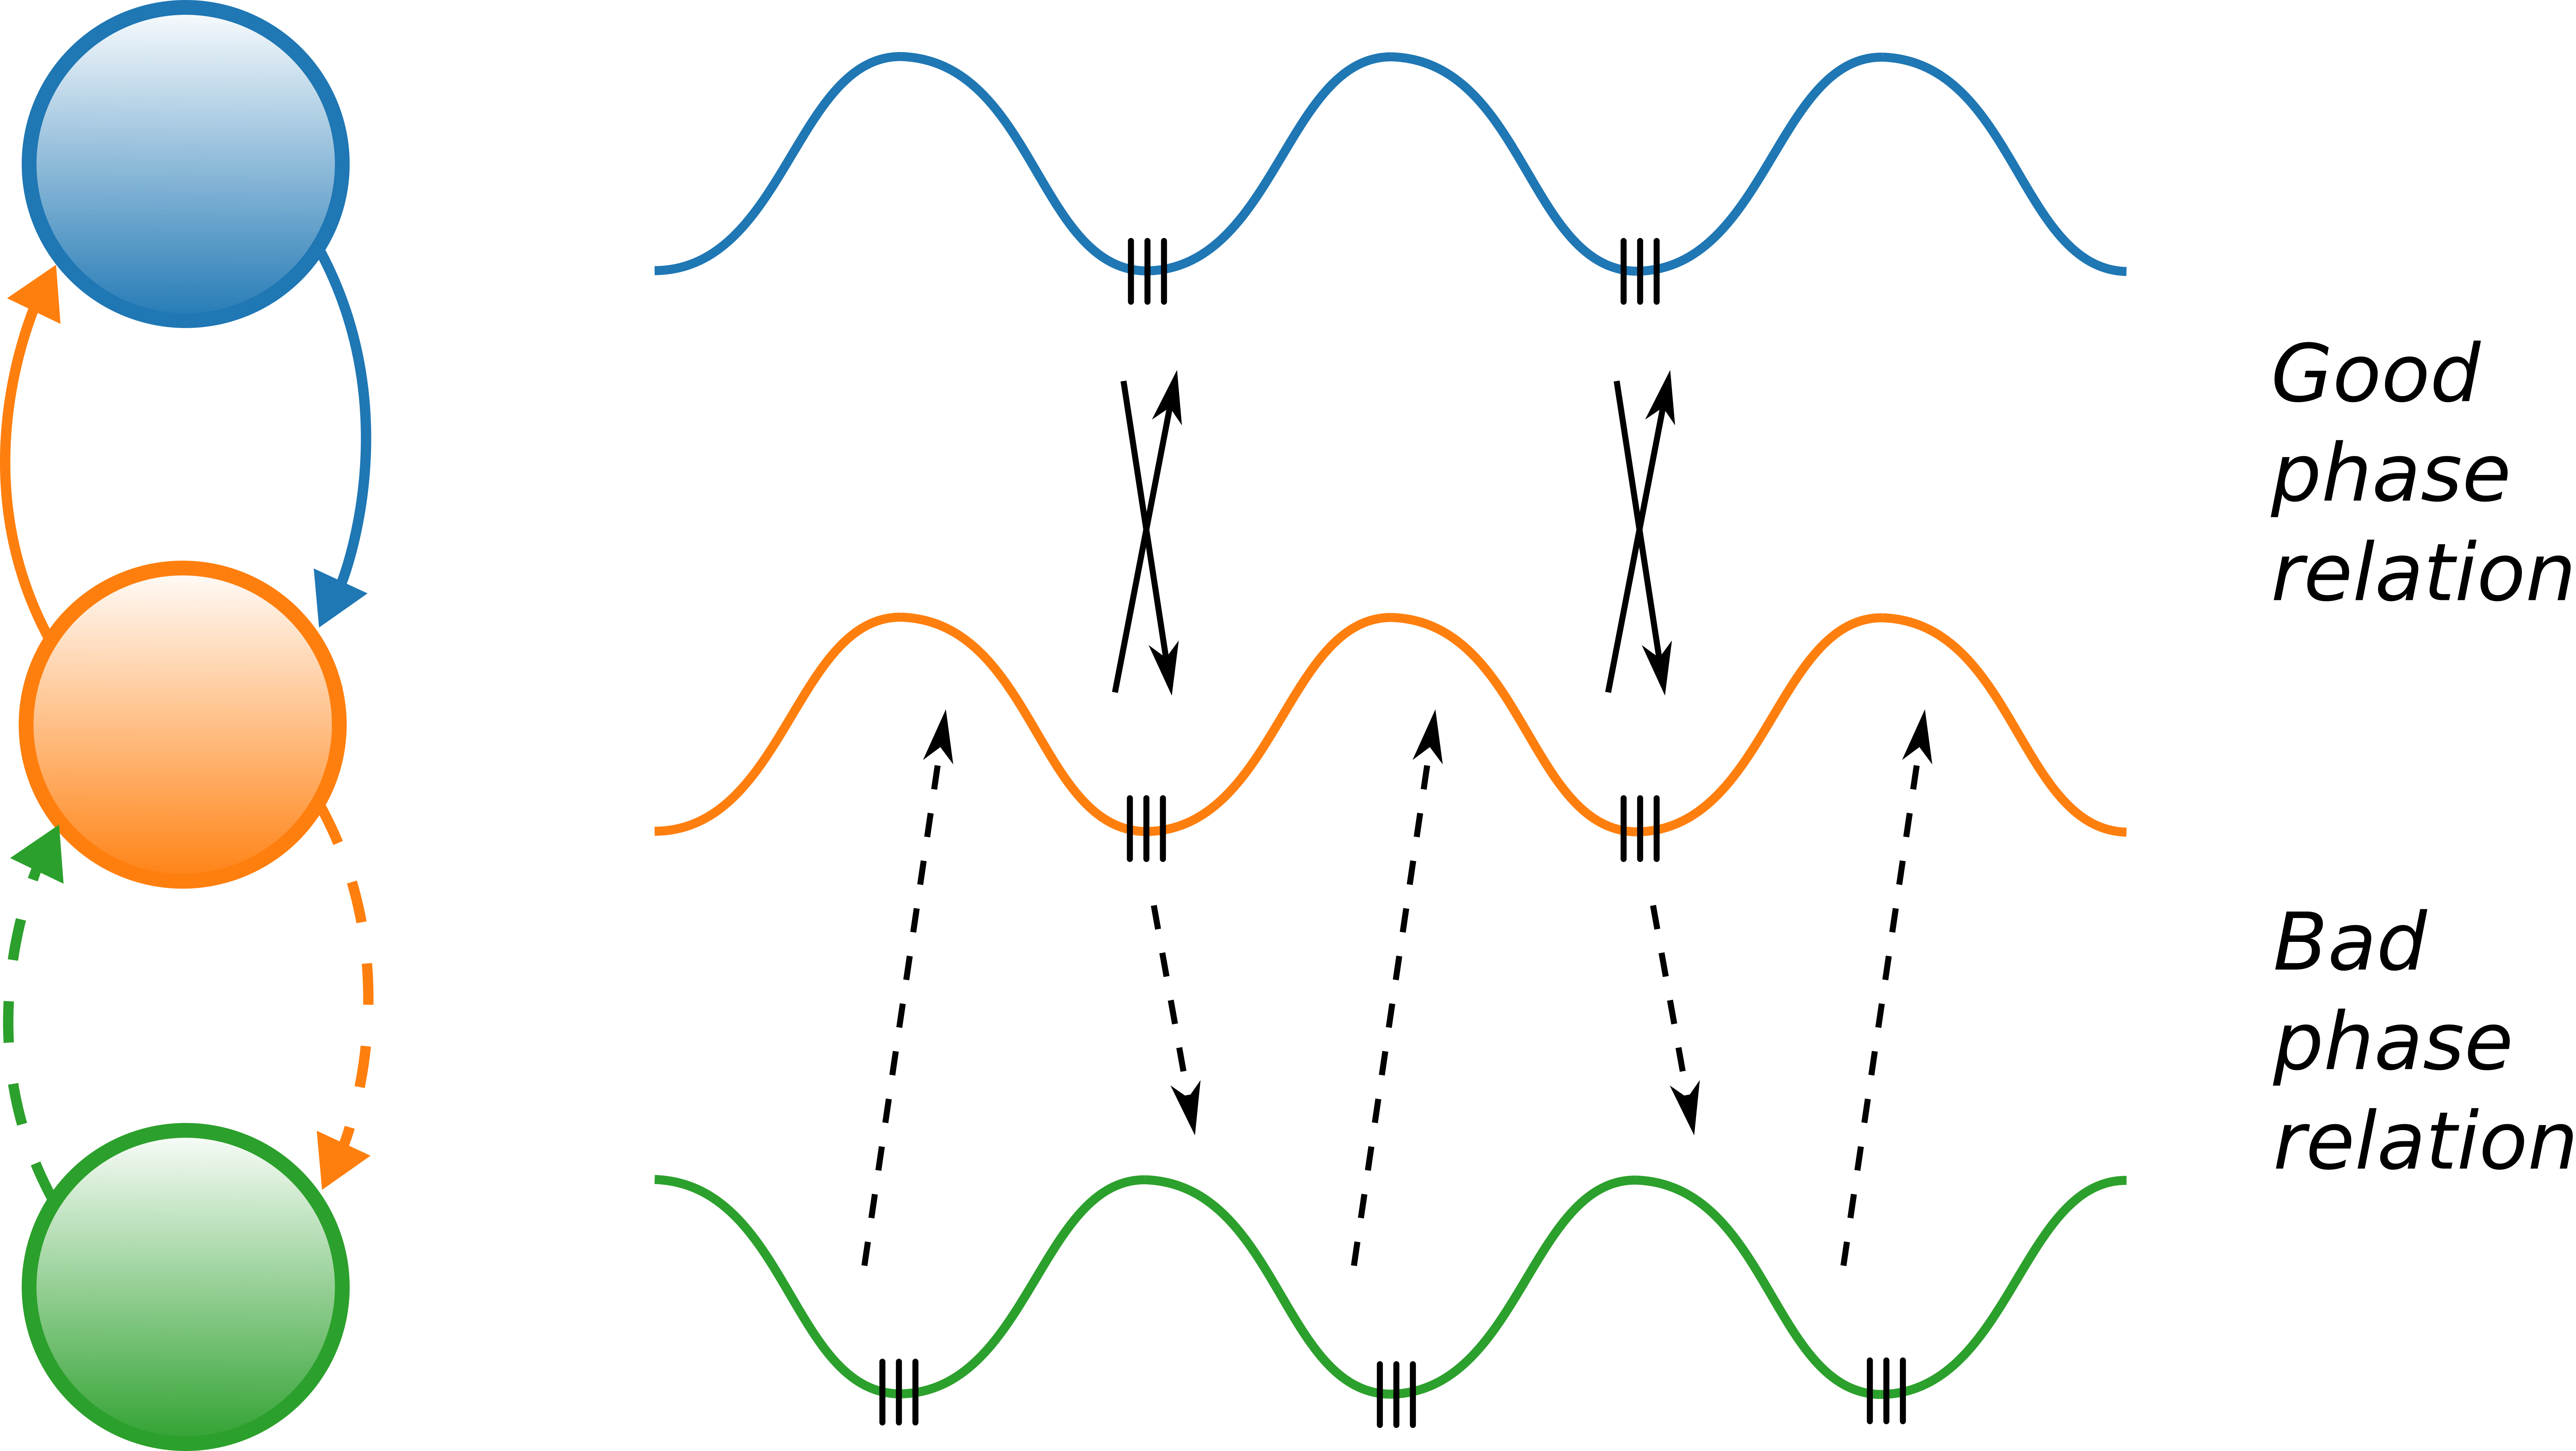
\includegraphics[width=0.75\textwidth]{chapter2/figures/coherence.png}
    \caption{\textbf{Neural communication through coherence}.
    Diagram illustrating three populations of neurons, each displaying rhythmic activity (LFP oscillations with spikes occurring during troughs).
    Effective communication occurs when time windows are aligned (blue and orange groups), while misalignment results in less effective communication (orange and green groups).
    Adapted from \citep{fries_mechanism_2005}.}
    \label{fig:CTC}
\end{figure}

Both CTC and BBS hypotheses are distinct but consistent with each other, and experiments supporting CTC have also provided strong evidence for the BBS hypothesis \citep{bosman2012attentional}.
While the BBS hypothesis primarily proposes a representational code, the CTC hypothesis delves into the mechanistic implications of neuronal oscillations on inter-neuronal communication.
The CTC hypothesis suggests that a dynamic communication framework lies at the core of our cognitive processes, with flexible neuronal coherence patterns serving as the adaptable neural foundation \citep{sancristobal_role_2014,fries_mechanism_2005,fries_rhythms_2015}.
\clearpage
\subsubsection{Information transmission in networks models}
CTC and BBS hypotheses motivated not only several experimental proposals \citep{bosman2012attentional,doi:10.1146/annurev.neuro.051508.135603,doi:10.1177/0959354307083492,MisselhornENEURO.0101-19.2019} but also computational studies \citep{battaglia_dynamic_2012,palmigiano_flexible_2017-1,pariz_high_2018, pariz_transmission_2021,vicente_dynamical_2008,gollo_dynamic_2010,gollo2011theta}.
% \textcolor{blue}{“Dynamical relaying can yield zero time lag neuronal synchrony despite long conduction delays”, R. Vicente, L. L. Gollo, C. R. Mirasso, I. Fischer and G. Pipa, Proceedings of the National Academy of Sciences USA 105, 17157, (2008);
% “Dynamic control for synchronization of separated cortical areas through thalamic relay”, L. L. Gollo, C. Mirasso and A. Villa, Neuroimage, 52, 947 (2010); 
% “Theta band zero-lag long-range cortical synchronization via hippocampal dynamical relaying”, L. L. Gollo, C. R. Mirasso, M. Atienza, M. Crespo-Garcia and J. L. Cantero, PLoS One 6, e17756 (2011);
% “Effect of the topology and delayed interactions in neuronal networks synchronization”, T. Pérez, G. C. García, V. M. Eguíluz, R. Vicente, G. Pipa and C. Mirasso, PLoS One 6, e19900 (2011). 147)	“Mechanisms of Zero-Lag Synchronization in Cortical Motifs”, L. L. Gollo, C. R. Mirasso, O. Sporns and M. Breakspear, PLoS Comput Biol 10(4): e1003548. doi:10.1371/journal.pcbi.1003548, (2014))}
It has been found that oscillators whose phase advances others act as leaders and efficiently transmit information to the laggard regions \citep{dalla2019exploring}.
A frequency mismatch, a relatively small difference in the oscillation frequency, can lead to a phase difference and directional information transfer, where the nodes with the highest frequency transmit information to those with the lowest frequency when the connection delay is ignored \citep{kirst_dynamic_2016,pariz_high_2018, pariz_transmission_2021}.
However, the interaction delay, caused by the finite time of signal transmission between nodes, is a key parameter that influences synchronization and phase relations between coupled oscillators 
\citep{ernst1995synchronization,ernst1998delay,yeung1999time,zeitler2009asymmetry,ko_phase-response_2009,esfahani_zero-lag_2014,mirasso_anticipated_2017}.
Since synchronization and phase relations determine effective routes for information transfer, and the properties of synchrony depend on the interaction delays, these delays play an important role in the emergence of communication patterns in neural circuits.
Thus, understanding the impact of transmission delays is essential to understanding information transmission in the brain.
Previous studies have focused mainly on two-component motifs, neglecting larger networks \citep{sancristobal_role_2014,barardi_phase-coherence_2014, kirst_dynamic_2016, palmigiano_flexible_2017-1, pariz_transmission_2021}.
Therefore, our interest lies in elevating the complexity to the next level by introducing a third node or oscillator to the motif, \textit{e.g.},  mimicking a cortico-thalamic-cortical circuit.
\subsection{Weakly-coupled oscillators: phase reduction}
To understand the emergence of synchronization in the brain, the study of coupled oscillators is essential, as it provides a theoretical framework that improves our understanding of collective behaviors in neural networks \citep{ashwin_mathematical_2016}.
Coupled oscillators refer to a collection of individual oscillating units or nodes that interact with each other through various forms of coupling.
Each oscillator exhibits its inherent rhythmic activity, but their mutual influence results in emergent behaviors and patterns at the network level \citep{schwemmer2012theory,KOKSALERSOZ201746,Mallada_2013}.
% A huge theoretical research in this field has laid the foundation for understanding synchronization in diverse brain regions, including the cortex, hippocampus, and thalamus, providing crucial insights into neural coding, information transfer, and cognitive functions. \textcolor{red}{CITAS}}

The concept of weak coupling has been a valuable asset in advancing our understanding of neuronal network synchronization, as evidenced by its application in various studies \citep{kuramoto1984phase,kopell2002mechanisms,izhikevich_dynamical_2007,schwemmer2012theory}.
This theory facilitates the reduction of complex dynamics within a network of interconnected neuronal oscillators to a more manageable set of equations that focus exclusively on the phase of each oscillator. This simplification allows for a more streamlined analysis of the system.

The phase reduction for collective network dynamics has been intensively investigated for analyzing the macroscopic synchronization properties between networks that show collective dynamics \citep{pikovsky2015dynamics}.
Using these methods, we can investigate a macroscopic phase sensitivity function and a macroscopic phase coupling function between networks.
Figure \ref{fig:phase_reduction_schematics} illustrates a framework where each network with collective oscillations, and many internal and external couplings, is reduced to a one-dimensional phase description.
Then, the derived macroscopic phase coupling function describes the effect of all external couplings between two networks on the phase
dynamics.
\begin{figure}[!htb]
    \centering
    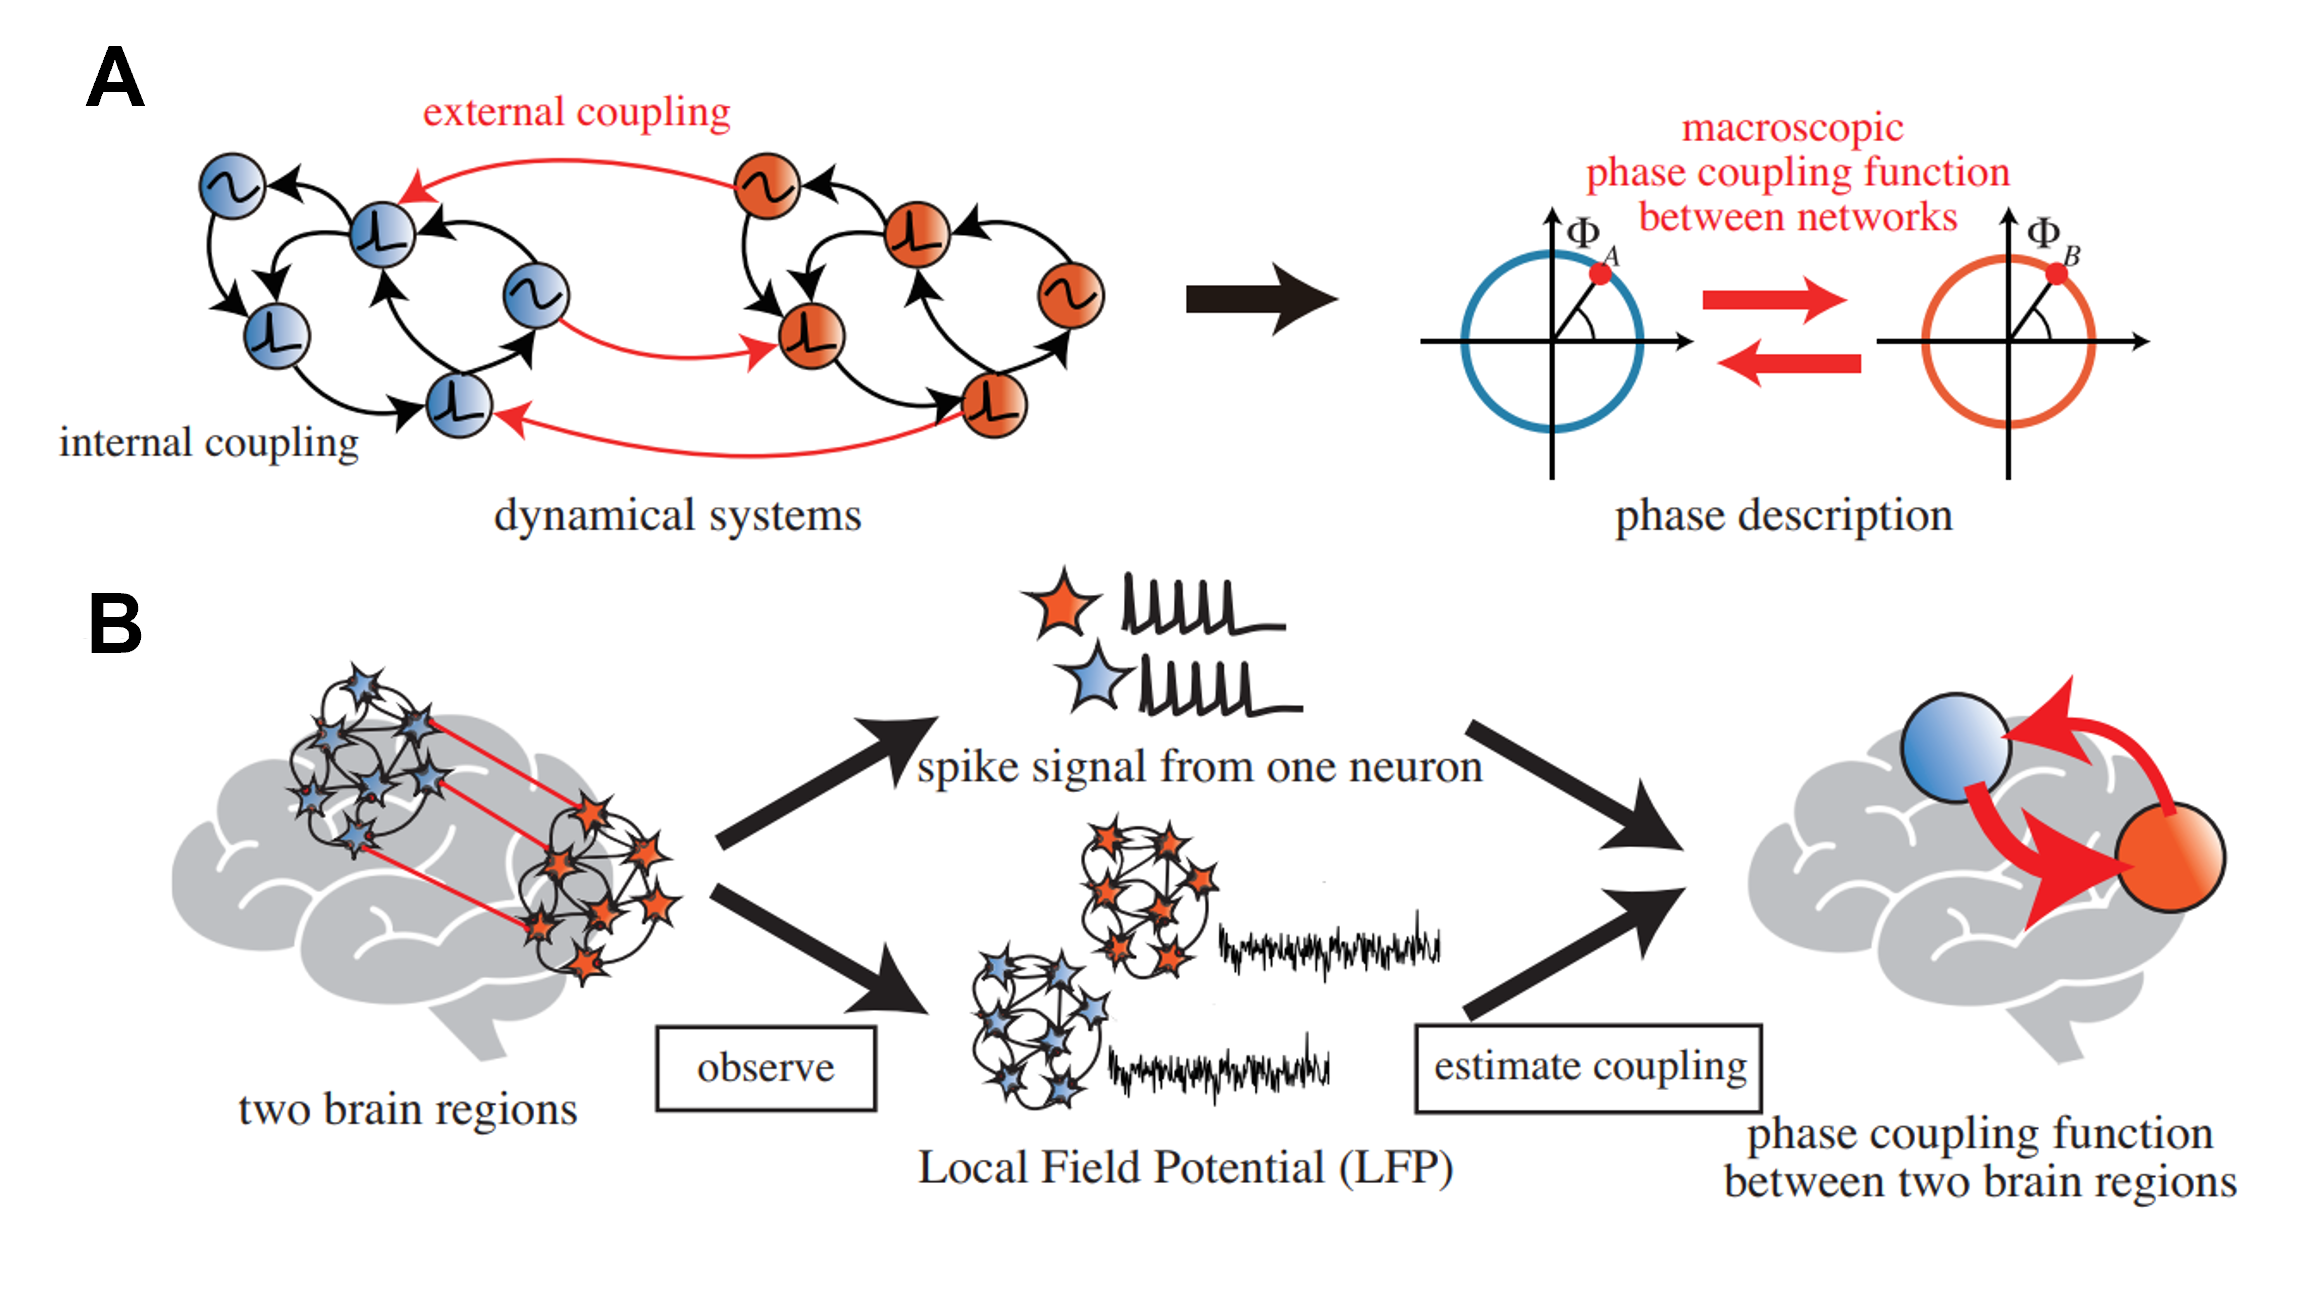
\includegraphics[width=\textwidth]{chapter2/figures/schematics_.png}
    \caption{\textbf{Phase reduction method}.
    % Schematic diagram of the phase reduction method for collective oscillation.
    Under conditions where stable limit cycles are established within each network and external couplings remain sufficiently weak, the dynamics of each network can be simplified to a single-phase equation (A).
    Illustration of the statistical inference process for determining connectivity between brain regions, wherein the dynamics of a brain region can be observed through metrics like the average membrane potential of neurons or local field potential (LFP).
    The phase coupling function is derived from observed time series data, although varying observation methods may yield different outcomes (B).
    Original figure from \citep{arai_extracting_2022}.}
    \label{fig:phase_reduction_schematics}
\end{figure}
\subsubsection{Network of networks}
Consider $N$ networks of $N_\gamma$ coupled dynamical nodes or units and weak interactions between the networks.
The dynamics of the node $i$ in network $\gamma$ is given by \citep{kirst_dynamic_2016}:
\begin{equation}
    \displaystyle\frac{d}{dt}\mathbf{x}_i^{\gamma} = \mathbf{f}_i^{\gamma}(\mathbf{x}_j{^\gamma}(t)) + \displaystyle\sum_{j\neq i}^{N_\gamma} \mathbf{g}_{ij}^\gamma(\mathbf{x}_i^\gamma(t),\mathbf{x}_i^\gamma(t)) + \varepsilon\displaystyle\sum_{\nu\neq\gamma}^{N}\displaystyle\sum_{j=1}^{N_\nu}\mathbf{h}_{ij}^{\gamma\nu}(\mathbf{x}_i^\gamma(t),\mathbf{x}(t)_j^\nu) + \mathbf{\eta}_i^\gamma(t),
    \label{eq:generic-network-of-networks}
\end{equation}
where $\mathbf{x}_i^{\gamma}(t)$ represents a $d_i^\gamma$-dimensional state of element $i$ in network $\gamma$ at time $t$, $\mathbf{f}_i^{\gamma}$ represents the individual dynamic of node $i$ in network $\gamma$, $\mathbf{g}_{ij}^{\gamma}$ represents the internal coupling from node $j$ to node $i$ in the network $\gamma$.
In this description, self-coupling is either omitted or assimilated into the term representing individual dynamics, \textit{i.e.}, $\mathbf{g}_{ii}^{\gamma} = \mathbf{0}$. 
The external coupling between networks is given by the vector function $\mathbf{h}_{ij}^{\gamma\nu}$.
The intensity of this interaction is determined by $\varepsilon$. 
The last term $\mathbf{\eta}_i^\gamma$ represents white Gaussian noise that every node receives.
The total dimension of that system would be $\sum_{\gamma=1}^{N}N_{\gamma}\dim(\mathbf{f}^{\gamma})$, where the dimension of $\mathbf{f}^{\gamma}$ depends on the oscillator model.

Assuming that each network has collective oscillation in a fully locked state and there is no perturbation, \textit{i.e.} $\varepsilon =0$ and $\mathbf{\eta}_i^\gamma = \mathbf{0}$, we can apply the phase reduction description to the dynamical system \eqref{eq:generic-network-of-networks} \citep{zahid2009predicting,lewis2013cooperative,pikovsky2015dynamics}.
In this scenario, the dynamics of node $i$ in the network $\gamma$ is assumed to exhibit periodic oscillations:
\begin{equation}
    \mathbf{x}_i^{\gamma}(t) = \mathbf{x}_i^{\gamma}(t+T_\gamma),
    \label{eq:phase-reduction}
\end{equation}
where each network exhibits a stable limit-cycle solution and $T_\gamma$ is the oscillation period of network $\gamma$.
Therefore, we can parameterize the dynamics by introducing the variable $\theta_\gamma(t) \in [0,2\pi)$. The state of the network $\gamma$ at time $t$ can be described as:
\begin{equation}
    \mathbf{x}_i^\gamma(t) = \mathbf{x}_i^\gamma(\theta_\gamma(t)),
\end{equation}
Then, the phase variable increases with a constant natural frequency $\Omega_\gamma$ as follows:
\begin{equation}
    \displaystyle\frac{d}{dt}\theta_\gamma(t) = \Omega_\gamma = \displaystyle\frac{2\pi}{T_\gamma}
    \label{eq:phase-reduction-2}
\end{equation}
Now, we assume that there is a perturbation in the system given by the coupling between networks, but this interaction is weak enough to keep the collective oscillatory dynamics on each network.
This is satisfied when $\varepsilon\ll 1$ and the noise intensity is also small.
Then, equation \eqref{eq:generic-network-of-networks} can be reduced to the following phase equation:
\begin{equation}
    \displaystyle\frac{d}{dt}\theta_\gamma(t) = \Omega_\gamma + \varepsilon\displaystyle\sum_{\nu\neq\gamma}\Gamma_{\gamma\nu}(\theta_\nu(t)-\theta_\gamma(t)) + \xi_\gamma(t),
     \label{eq:phase-reduction-3}
\end{equation}
where $\Gamma_{\gamma\nu}$ represents the phase coupling functions between networks $\nu$ and $\gamma$ and depends of the phase differences only.
This function is obtained by averaging the product of phase sensitivity function and external coupling throughout the collective oscillation \citep{kirst_dynamic_2016}.
It only depends on the phase difference $\theta_\nu-\theta_\gamma$, which represents the effect of all external couplings from network $\nu$ to network $\gamma$.
The independent white Gaussian noise $\xi_\gamma(t)$ given to the network $\gamma$ satisfies $\langle \xi_\gamma(t)\rangle = 0$ and $\langle \xi_\gamma(t)\xi_\nu(s) \rangle = 2D_\gamma\delta_{\gamma\nu}\delta(t-s)$,
where $\delta_{\gamma\nu}$ and $\delta(t)$ are the Kronecker delta and Dirac delta functions, respectively.
This noise term represents the effect of all the noise $\mathbf{\eta}_i^\gamma(t)$ given to the network $\gamma$.
This parameterization allows a considerable reduction of the system dimension from $\sum_{\gamma=1}^{N}N_{\gamma}\dim(\mathbf{f^\gamma})$ to $N$.
Moreover, additional dimension reduction can be achieved when examining relative phase differences $\theta_{\gamma\nu}(t) = \theta_\nu(t) -\theta_\gamma(t)$, giving rise to a dimension of $N-1$, then:
% Further dimension reduction is achieved when considering the dynamics of the phases differences $\Delta\theta_{\gamma\nu}(t) = \theta_\nu(t)-\theta_\gamma(t)$, then
\begin{equation}
    \begin{aligned}
    \displaystyle\frac{d}{dt}\theta_{\gamma\nu}(t) = \Delta\Omega_{\gamma\nu}+\varepsilon\displaystyle\sum_{\nu\neq\gamma}\Big( \Gamma_{\gamma\nu}(\theta_{\gamma\nu}(t))-\Gamma_{\nu\gamma}(\theta_{\nu\gamma}(t))\Big) = \\
    \Delta\Omega_{\gamma\nu}+\varepsilon\displaystyle\sum_{\nu\neq\gamma}\Big( \Gamma_{\gamma\nu} (\theta_{\gamma\nu}(t))-\Gamma_{\nu\gamma}(-\theta_{\gamma\nu}(t))\Big),
    \label{eq:phase-reduction-4_}
    \end{aligned}
\end{equation}
where $\Delta\Omega_{\gamma\nu} = \Omega_\nu-\Omega_\gamma$.
This phase reduction method is applicable to more complex models, including multicompartment neuron models, resulting in a significantly larger dimension reduction \citep{zahid2009predicting,lewis2013cooperative}.

In the previous section, we mentioned the importance of delays in brain circuits, and therefore, we can incorporate them in the  equation \eqref{eq:phase-reduction-3} to obtain:
\begin{equation}
\displaystyle\frac{d}{dt}\theta_\gamma(t) = \Omega_\gamma + \varepsilon\displaystyle\sum_{\nu\neq\gamma}\Gamma_{\gamma\nu}\big(\theta_\nu(t-\tau_{\nu\gamma})-\theta_\gamma(t)\big) + \xi_\gamma(t),
     \label{eq:phase-reduction-5}
\end{equation}
where $\tau_{\nu\gamma}$ is the delay from oscillator $\nu$ to oscillator $\gamma$. 
Once more, we can contemplate the phase difference, but a prerequisite will be imposed before proceeding.
Since we are interested in synchronized or phase-locked states, we impose to each oscillator dynamics to be:
\clearpage
\begin{equation}
    \theta_{\gamma}(t) = \theta_0(t) + \delta_\gamma,
\end{equation}
where $\delta_\gamma$ is a constant phase and we are considering an ideal case where the noise is neglected.
This means that all phase oscillators are described from a phase reference $\theta_0$.
Along the phase-locked solutions, the effect of a time delay on the connections between oscillators $\gamma$ and $\nu$  translates into a constant phase $\delta_{\nu\gamma}$ shift \citep{mirasso_anticipated_2017}:
\begin{equation}
\begin{aligned}
    \displaystyle\frac{d}{dt}\theta_\gamma(t)  &= \Omega_\gamma + \varepsilon\displaystyle\sum_{\nu\ne\gamma}\Gamma_{\gamma\nu}\big( \theta_\nu(t)-\theta_\gamma(t)-\delta_{\nu\gamma}\big)\\
    \quad &= \Omega_\gamma +\varepsilon\displaystyle\sum_{\nu\ne\gamma}\Gamma_{\gamma\nu}\big( \theta_{\nu\gamma}(t)-\delta_{\nu\gamma}\big),
\end{aligned}
    \label{eq:phase-reduction-6}
\end{equation} 
where $\delta_{\nu\gamma} = \Omega_\nu\tau_{\nu\gamma}$.

The complexity of the function ${\Gamma}$ varies depending on the model used to describe the dynamics of $\theta_\gamma(t)$. 
Several theoretical advancements in synchronization exist where a specific model may not have been explicitly defined, but rather, certain conditions have been impose on the function $\Gamma$ \citep{Mallada_2013,esfahani_zero-lag_2014,sadeghi_synchronization_2014,KOKSALERSOZ201746,pariz_transmission_2021}.
Other scenarios require numerical analysis for this phase reduction method.
However, from a theoretical perspective, in this study, we will consider the simplest case which arises by imposing $\varepsilon\Gamma_{\nu\gamma}(\cdot) = K_{\nu\gamma}\sin(\cdot)$, leading to the Kuramoto model.
With this definition, the parameter $\varepsilon$, which determines the level of interaction between the oscillators, becomes encapsulated within the set of coupling constants $\{K_{\nu\gamma}\}$.
Therefore, equation \eqref{eq:phase-reduction-6} is simplified to:
\begin{equation}
    \displaystyle\frac{d}{dt}\theta_\gamma(t) = \Omega_\gamma + \sum_{\nu\ne\gamma}K_{\nu\gamma}\sin\big(\theta_\nu(t)-\theta_\gamma(t)-\delta_{\nu\gamma}\big),
    \label{eq:phase-reduction-kuramoto}
\end{equation}
This simplification, allows us to analyze, in a first approximation, the expected behavior of the motifs under study.
It allows us to determine the expected behavior in terms of synchronization depending on the different conditions of the system, such as the delays and the coupling constant between the oscillators.
Here, we will explore two simple cases that provide valuable insights: the first involves two bidirectionally coupled oscillators, referred to as a 2-motif for simplicity, and the V-motif, which is one of the motifs of interest for studying information transmission.
In particular, its synchronization-related properties have previously been studied \citep{esfahani_zero-lag_2014,sadeghi_synchronization_2014,gollo_dynamic_2010,mirasso_anticipated_2017,pariz_high_2018}.
\clearpage
\subsection{Synchronization in motifs}
Here, we will discuss the synchronization states or phase-locked states of the aforementioned motifs: the 2-motif and the V-motif.
%These examples allowed us to predict the behavior of the networks of networks.
The feasibility of these solutions relies on the intricate interplay between delays and coupling constants, shaping the parameter space.

\subsubsection{2-motif}
The 2-motif circuit consists of two mutually coupled oscillators and, then, its dynamics is captured by the phase difference between the two oscillators $\theta_{12}(t) = \theta_1(t)-\theta_2(t)$.
Applying equation \eqref{eq:phase-reduction-kuramoto}, the dynamics of the 2-motif is described by:
\begin{equation}
    \displaystyle\frac{d}{dt}{\theta}_{12}(t) = \Delta\Omega_{12} + K_{21}\sin(-\theta_{12}-\delta_{21}) - K_{12}\sin(\theta_{12}-\delta_{12}), 
    \label{eq:2motif}
\end{equation}
The simplest case is to consider the symmetric scenario where both oscillators have the same intrinsic frequency, $\Omega = \Omega_1 = \Omega_2$, the constant coupling are equal $K=K_{12}=K_{21}$, and the delay of both couplings are also identical $\delta = \delta_{12}=\delta_{21}$.
Then, equation \eqref{eq:2motif} becomes:
\begin{equation}
    \displaystyle\frac{d}{dt}{\theta}_{12}(t) = -2K\cos\delta\sin\theta_{12},
    \label{eq:2motif-symmetric}
\end{equation}
whose asymptotically fixed points are 
\begin{equation}
    \begin{aligned}
        \theta_{12} &= 0, \hspace{1cm}\delta\in\bigg[0,\displaystyle\frac{\pi}{2}\bigg) \cup\bigg[\displaystyle\frac{3\pi}{2},2\pi\bigg), \\
        \theta_{12} &= \pi, \hspace{1cm} \delta\in \bigg[\displaystyle\frac{\pi}{2},\displaystyle\frac{3\pi}{2}\bigg),
    \end{aligned}
\end{equation}
\begin{figure}[!htb]
\centering
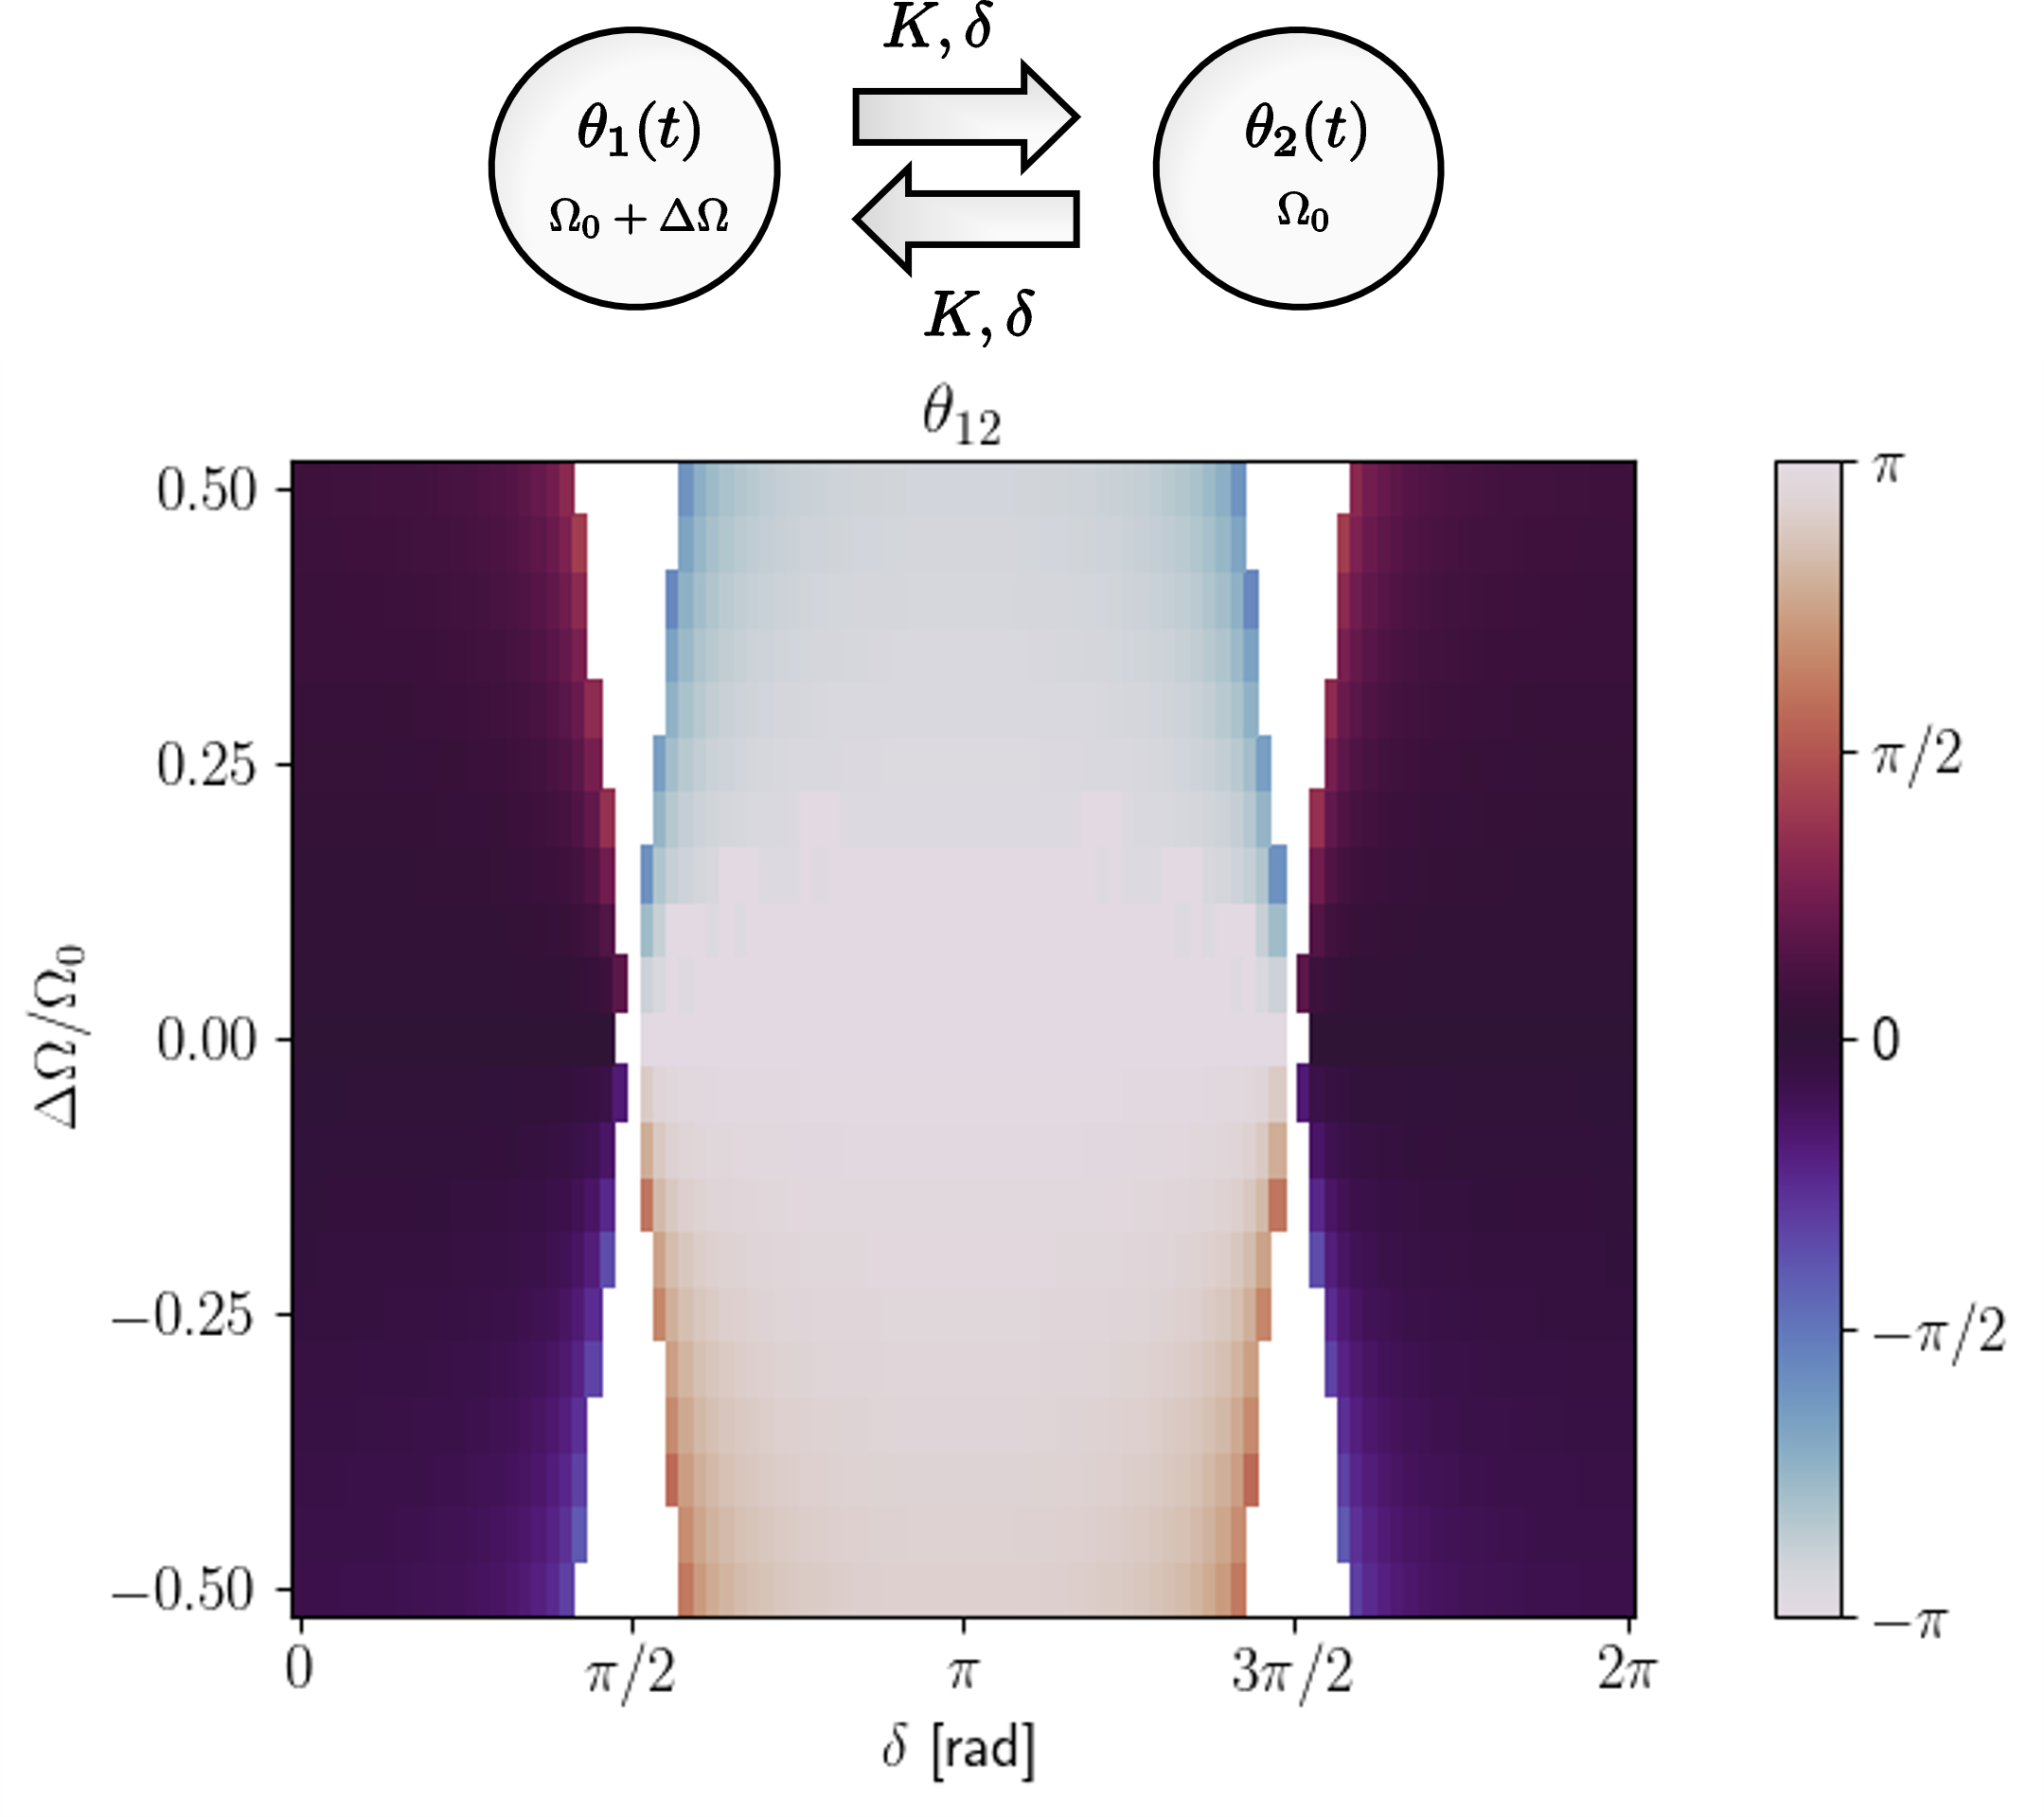
\includegraphics[width=0.7\textwidth]{chapter2/figures/2motif_different_omega_edited.png}
    \caption{\textbf{2-motif: phase-locked solutions.} Asymptotically stable fixed points solutions as function of the the frequency mismatch $\Delta\Omega$ applied into one of the two nodes and the common delay between them. White regions indicate region of unstable fixed points. Note that the colormap chosen is periodic in the sense that color associated to $-\pi$ coincides to the one of $\pi$.}
    \label{fig:2motif-syncrhonization}
\end{figure}
So, depending on the delay, the dynamics of the oscillators are in-phase or anti-phase.
The addition of an inhomogeneity breaks the symmetry and, therefore, new configurations start to emerge \citep{sadeghi_synchronization_2014,esfahani_zero-lag_2014}.
In Figure \ref{fig:2motif-syncrhonization} we show the case in which the inhomogeneity has been added by imposing a frequency mismatch $\Omega' = \Omega +\Delta\Omega$ on one of the oscillators.
Let us assume that this oscillator is oscillator 1.
For small values of $\Delta\Omega$, the system exhibits the same two fixed points, either in-phase or anti-phase solutions.
An increase in the frequency mismatch has several effects. Initially, in areas where the system displayed in-phase dynamics, it now manifests a consistent non-zero phase difference.
When the intrinsic frequency of oscillator 1 is higher, it leads oscillator 2, whereas when the intrinsic frequency of oscillator 1 decreases, oscillator 2 leads oscillator 1.
An opposite effect occurs in regions where the oscillators were initially in anti-phase dynamics.
As the intrinsic frequency of oscillator 1 increases, oscillator 2 leads oscillator 1, and vice versa.
Another effect of this frequency mismatch is the emergence of instability regions, where the fixed points of the system are not asymptotically stable (white regions).
These unstable regions start to appear in the discontinuity where the stable phase-locked solutions change from $0$ to $\pi$ and vice versa, as a function of the phase $\delta$.
The delay interval for these unstable solutions increases as the frequency mismatch increases.
Therefore, delay plays a significant role in shaping the relative dynamics between coupled oscillators when the system exhibits inhomogeneity.

\subsubsection{V-motif}
The introduction of a third oscillator into the system allows for the description of the entire system through the dynamics of two phase differences $\theta_{12}(t)$ and $\theta_{13}(t)$, since the third one $\theta_{23}(t)$ can be described as a linear combination of the other two.
The general equation for a C-motif consisting in three mutually-coupled oscillators is given by:
\begin{equation}
\begin{aligned}
    \displaystyle\frac{d}{dt}\theta_{12}(t) & = \Delta\Omega_{12} + K_{21}\sin(-\theta_{12}-\delta_{21}) + K_{31}\sin(-\theta_{13} - \delta_{31})\\
       & \quad - K_{12}\sin(\theta_{12}-\delta_{12}) - K_{32}\sin(\theta_{12}-\theta_{13}-\delta_{32}), \\
    \displaystyle\frac{d}{dt}\theta_{13}(t) & = \Delta\Omega_{13} + K_{21}\sin(-\delta_{12}-\delta_{21}) + K_{31}\sin(-\theta_{13} - \delta_{31}) \\
    & \quad -K_{13}\sin(\theta_{13}-\delta_{13}) - K_{23}\sin(\theta_{13}-\theta_{12}-\delta_{23}).
    \label{eq:vmotif}
\end{aligned}
\end{equation}
By imposing the coupling constants between the outer nodes $k_{13}=k_{31}=0$, we obtained the equations for the V-motif.

Considering the symmetric scenario $K = K_{12} = K_{21} = K_{23} = K_{32}$, $\delta = \delta_{12} = \delta_{21} = \delta_{23} = \delta_{32}$, and $\Omega = \Omega_1 = \Omega_2 = \Omega_3$, equation \eqref{eq:vmotif} reduces to:
\begin{equation}
    \begin{aligned}
    \displaystyle\frac{d}{dt}\theta_{12}(t) &= K\sin(-\theta_{12}-\delta) - K\sin(\theta_{12}-\delta)- K\sin(\theta_{12}-\theta_{13}-\delta), \\
    \displaystyle\frac{d}{dt}\theta_{13}(t) &= K\sin(-\theta_{12}-\delta)-
    K\sin(\theta_{13}-\theta_{12}-\delta),
    \end{aligned}
    \label{eq:vmotif-symmetric}
\end{equation}
whose asymptotically stable fixed points are given by \citep{mirasso_anticipated_2017}: 
\begin{equation}
    \begin{cases}
        \theta_{13} = 0\\
        \theta_{12} = \arctan\bigg(\displaystyle\frac{\tan\delta}{3}\bigg) 
    \end{cases},
        \quad \delta\in\bigg[0,\displaystyle\frac{\pi}{3}\bigg)\cup\bigg[\displaystyle\frac{2\pi}{3},\displaystyle\frac{4\pi}{3}\bigg)\cup
        \bigg[\displaystyle\frac{5\pi}{3},2\pi\bigg).
\end{equation}
Zero-lag synchronization between the outer oscillators is a stable solution of the system, independently of the delay (in the stable interval).
However, the system has other solutions where these nodes are in anti-phase, but they are not stable \citep{mirasso_anticipated_2017}.
The delay interval given by $[\pi/3,2\pi/3)\cup[4\pi/3,5\pi/3]$ is the unstable region where none of the solutions are stable.
The emergence of this region is not exclusive of the Kuramoto model since similar behaviors have been observed using other neural models such as Hodgkin-Huxley or Izhikevich \citep{mirasso_anticipated_2017} or neural networks with integrate-and-fire neurons \citep{gollo_dynamic_2010}.
Therefore, it is a characteristic of the structure of the topology rather than the model.
Nevertheless, the occurrence of the unstable region may vary across different delay intervals, contingent on the class (I or II) to which those oscillators belong \citep{sadeghi_synchronization_2014}.

Now, we add an inhomogeneity through a frequency mismatch denoted by $\Delta\Omega$.
In Figure \ref{fig:vmotif-synchronization} we show the phase-locked solution of the V-motif. 
\begin{figure}[!htb]
    \centering
    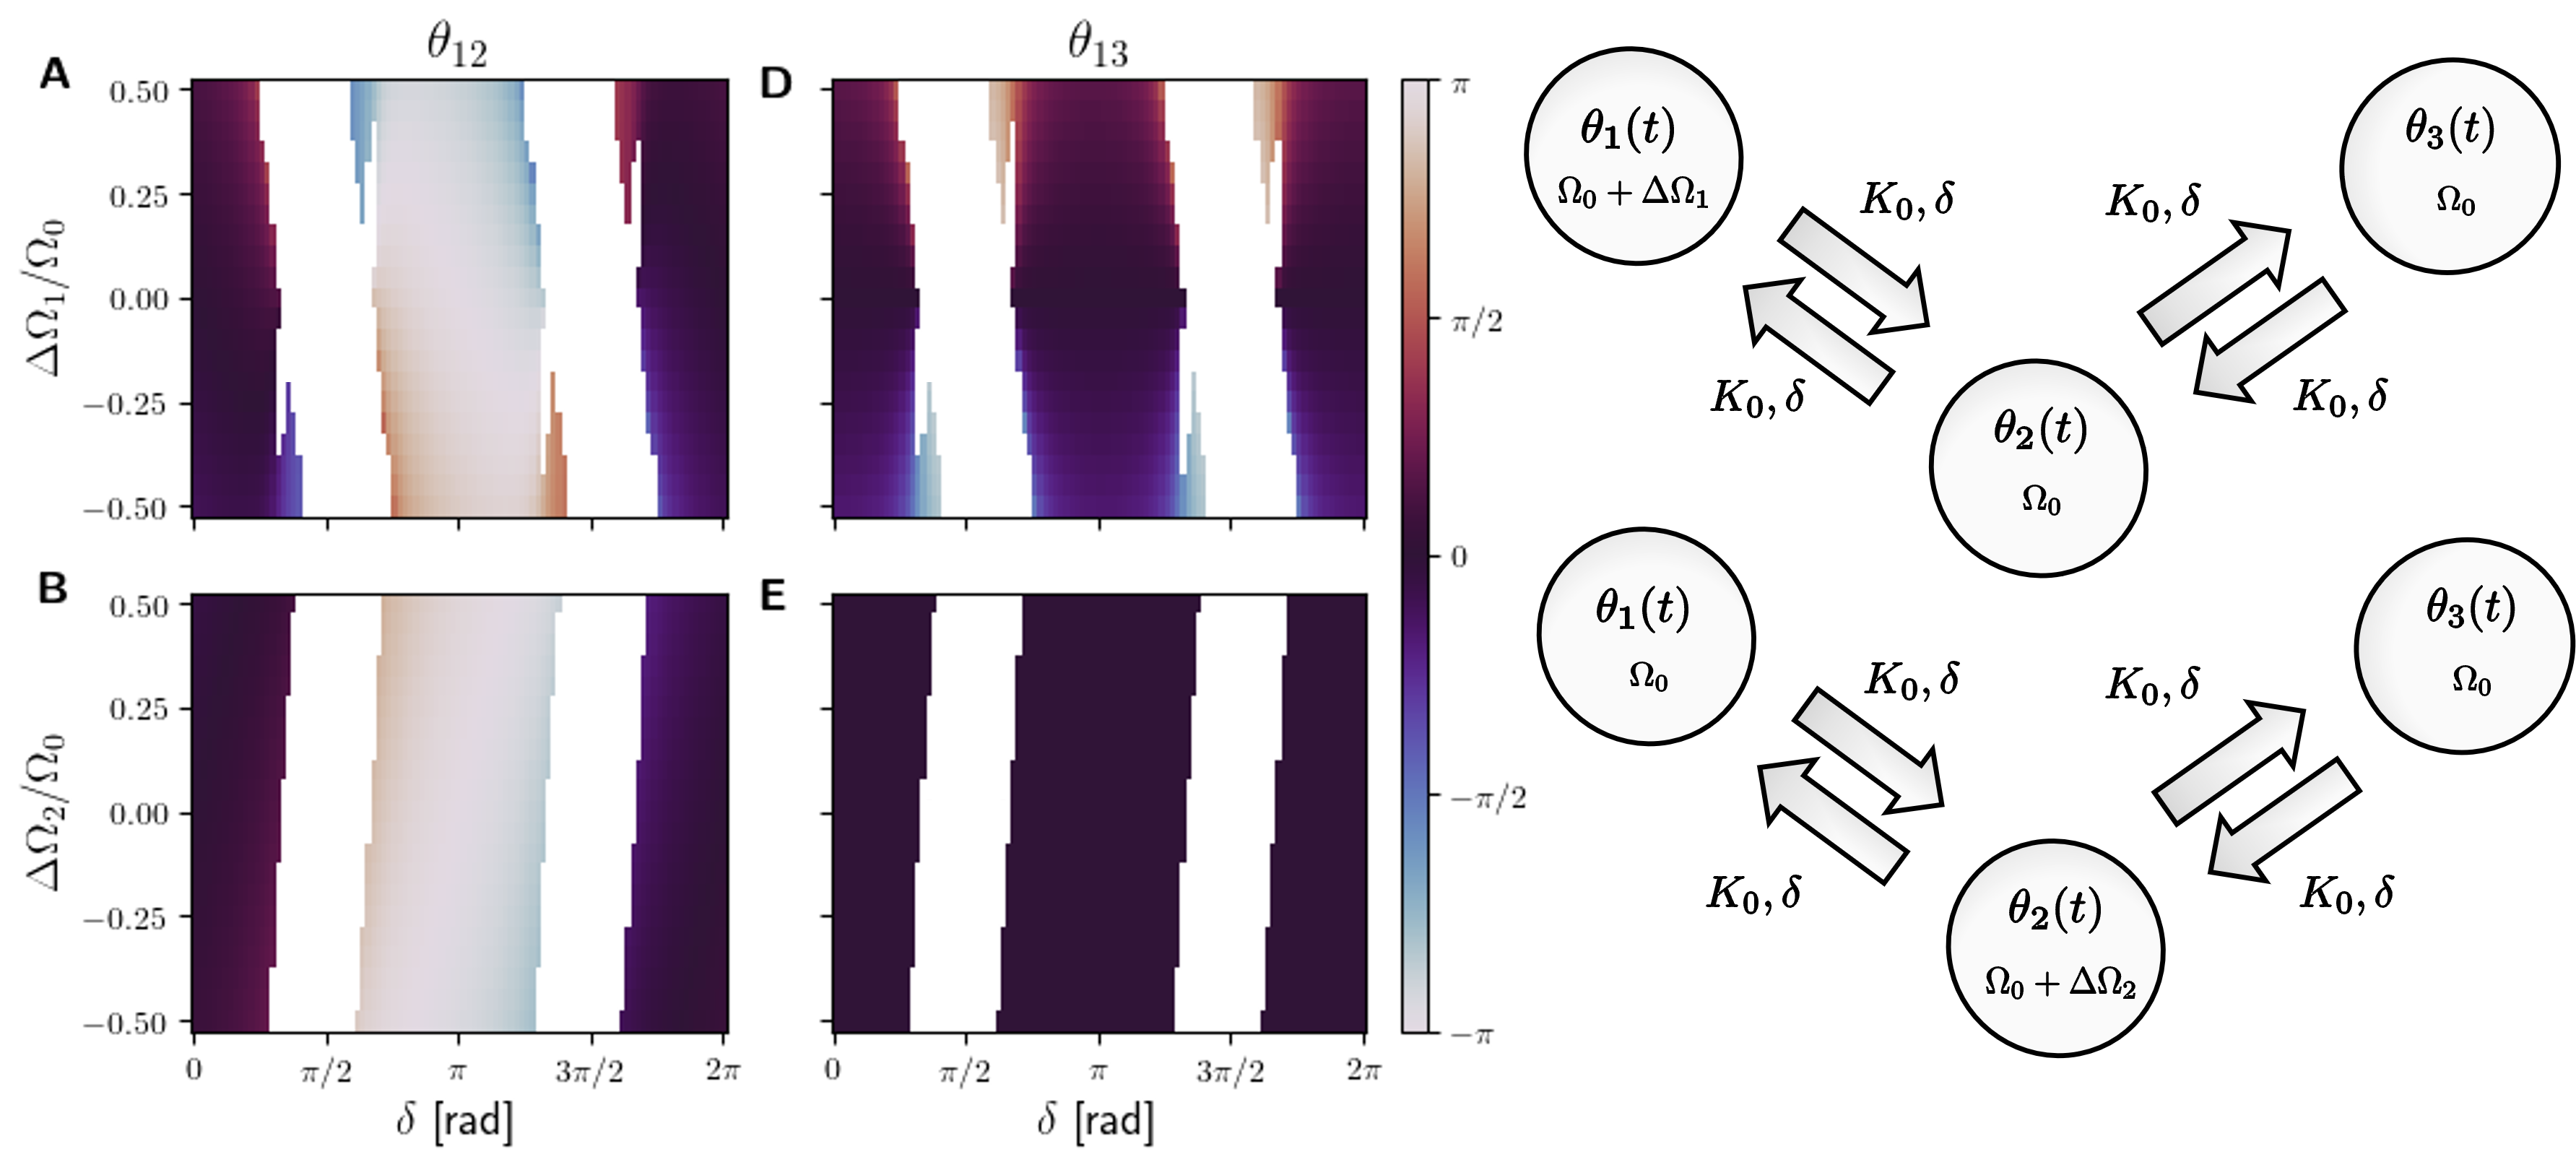
\includegraphics[width=\textwidth]{chapter2/figures/vmotif_same_omega_edited.png}
    \caption{\textbf{V-motif: phase-locked solutions}.
    Panels A and B indicate the asymptotically stable fixed points of $\theta_{12}(t)$ and $\theta_{13}(t)$, respectively. as function of the frequency mismatch $\Delta\Omega_1$ applied in one of the outer oscillators. Similarly, panels C and D show the asymptotically stable fixed points when the frequency mismatch $\Delta\Omega_2$ is applied in the central oscillator.
    White regions indicate the unstable regions, \textit{i.e.}, where the fixed points are unstable.}
    \label{fig:vmotif-synchronization}
\end{figure}
There are two scenarios, the first (top) when this frequency mismatch $\Delta\Omega_1$ is applied in one of the outer oscillators, oscillator 1, and the second (bottom) when the frequency mismatch $\Delta\Omega_2$ is applied in the center oscillator, oscillator 2.
The boundary of stable regions shifts based on both frequency and delay, varying according to the oscillator with a distinct intrinsic frequency.

Like in the case of the 2-motif, when the frequency mismatch increases positively, oscillator 1 tends to advance oscillator 2 and also oscillator 3, for small and large delays. 
The opposite happens in the stable intermediate region where oscillator 1 and oscillator 2 are initially in anti-phase, and it is oscillator 2 that advances over both oscillators 1 and 3.
However, when the frequency mismatch is applied to the central oscillator, the symmetry of the system is kept, and then, the system exhibits zero-lag synchronization between oscillator 1 and 3 independently of the inhomogeneity \citep{esfahani_zero-lag_2014}.


\subsection{Objectives}
As previously mentioned, motifs serve as fundamental circuits that depict functional interactions within distinct brain regions.
For example, the V-motif could represent a cortico-thalamo-cortical circuit.
Our aim was to evaluate the efficiency of this circuit, characterized by zero-time synchronization, in transmitting information and to discern the associated conditions.
This study builds upon previous research \citep{pariz_transmission_2021}, which investigated a similar question concerning two bidirectionally coupled populations, what we have called the 2-motif.

Another objective is to elucidate the significance of cortico-cortical connections, leading to the formation of the C-motif.
To achieve this, we employed a network of networks model and utilize information theory measures to quantify the outcomes.
\end{document}